\chapter{Ex-Vivo Renal MRI}
\label{chap:ex}

\begin{abstract}
	This work was presented as a digital poster at the \ac{ISMRM} 27th Annual Meeting 2019 \cite{daniel_effects_2019} and as a poster at \ac{UKKW} 2019 \cite{kazmi_determining_2019}.
\end{abstract}
\acresetall
\section{Introduction}

A recurring theme in renal \ac{MRI} studies are the limitations imposed by respiratory motion. Sequences must either be optimised and accelerated to fit within a breath-hold, be hugely slowed down through the use of respiratory triggering or accept the motion artefacts that are inevitable during free-breathing acquisition. Additionally the common trade-off in \ac{MRI} between voxel size, \ac{FOV} and acquisition time become all the more limiting within the constraints of respirator motion. While these issues are ever-present in day-to-day clinical practice, they also imped progress, and ultimately, clinical adoption, of techniques in the research phases of their development. Often in research, it is desirable to acquire data of higher quality than would be required in clinical practice.

\subsection{Validation of Multiparametric MRI via a Nephrectomy Model}

\subsection{Assessment of Allograft Viability}

\section{MRI Protocol Development}

\begin{figure}[H]
	\centering
	\includegraphics[width=0.5\textwidth]{Neph/head_coil.jpg}
	\caption{A sample sat within the 32 channel 3T head coil. A bespoke ex-vivo sample coil would have less space between the coil and the sample.}
	\label{fig:ex_head_coil}	
\end{figure}

\subsection{\tone Mapping}
% Acquisition
\begin{figure}[H]
	\centering
	\includegraphics[width=1\textwidth]{Neph/Individual_TI.eps}
	\caption{Acquisitions at each of the \ac{TI} at 7T.}
	\label{fig:ex_ir_data}	
\end{figure}
% smodding
\begin{figure}[H]
	\centering
	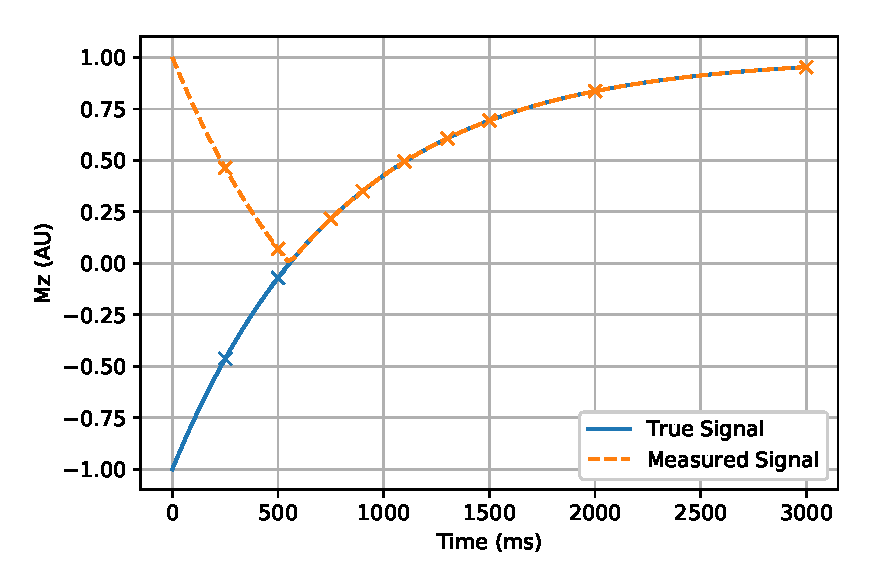
\includegraphics[width=0.5\textwidth]{neph/signal_correction.eps}
	\caption{A simulation of the true and measured magnetisation for a $T_1$ of 800 ms. The crosses represent the inversion times at which the inversion recovery is sampled.}
	\label{fig:ex_sig_mag_correction}	
\end{figure}
% Post Processing

\begin{figure}[H]
	\centering
	\begin{subfigure}[c]{0.47\textwidth}
		\centering
		\includegraphics[width=1\textwidth]{Neph/T1_map_3T.eps}
		\caption{}
		\label{fig:ex_t1_map_3t}
	\end{subfigure}
	\hfill
	\begin{subfigure}[c]{0.47\textwidth}
		\centering
		\includegraphics[width=1\textwidth]{Neph/T1_map_7T.eps}
		\caption{}
		\label{fig:ex_t1_map_7t}
	\end{subfigure}
	\caption{(\subref{fig:ex_t1_map_3t}) \tone map of a kidney twenty four hours after fixation at 3 T. (\subref{fig:ex_t1_map_7t}) \tone map twenty four hours after fixation at 7 T  }
	\label{fig:ex_t1_maps}
\end{figure}

\subsection{\ttwo Mapping}
% Acquisition
% Post processing

\subsection{\ttwostar Mapping}
% Acquisition
\begin{figure}[H]
	\centering
	\includegraphics[width=0.8\textwidth]{Neph/Individual_TE.eps}
	\caption{Acquisitions at each of the \ac{TE} at 7T.}
	\label{fig:ex_t2star_raw_data}	
\end{figure}
% Post processing
% Fitting methods

\begin{figure}[H]
	\centering
	\begin{subfigure}[c]{0.47\textwidth}
		\centering
		\includegraphics[width=1\textwidth]{Neph/T2star_map_3T.eps}
		\caption{}
		\label{fig:ex_t2star_map_3t}
	\end{subfigure}
	\hfill
	\begin{subfigure}[c]{0.47\textwidth}
		\centering
		\includegraphics[width=1\textwidth]{Neph/T2star_map_7T.eps}
		\caption{}
		\label{fig:ex_t2star_map_7t}
	\end{subfigure}
	\caption{(\subref{fig:ex_t2star_map_3t}) \ttwostar map twenty four hours after fixation at 3 T. (\subref{fig:ex_t2star_map_7t}) \ttwostar map twenty four hours after fixation at 7 T.}
	\label{fig:ex_t2star_maps}
\end{figure}

\subsection{\acl*{ADC} Mapping}
% Acquisition
% Distortion correction
% Post processing

\subsubsection{Optimising b-values}


\subsection{\acl*{DTI}}
% Acquisition
% Distortion Correction
% Processing (FA and Tractography)
\begin{figure}[H]
	\centering
	\includegraphics[width=.9\textwidth]{Other/DTI/img5c.png}
	\caption{Example tractography generated using the above protocol.}
	\label{fig:ex_dti_tracts}
\end{figure}

\begin{figure}[H]
	\centering
	\includegraphics[width=.55\textwidth]{Other/DTI/dti_FA.png}
	\caption{An example \ac{FA} map generated using the protocol above.}
	\label{fig:ex_dti_fa}
\end{figure}

\section{Optimising Tissue Fixation}
% Motivation
% Results
\begin{figure}[H]
	\centering
	\begin{subfigure}[c]{0.9\textwidth}
		\centering
		\begin{subfigure}[c]{0.47\textwidth}
			\centering
			\includegraphics[width=0.9\textwidth, angle=180]{neph/meat_kidney}
			\caption{}
			\label{fig:ex_samples_meat_kidney}
		\end{subfigure}
		\hfill
		\begin{subfigure}[c]{0.47\textwidth}
			\centering
			\includegraphics[width=0.9\textwidth, angle=180]{neph/sb_kidney}
			\caption{}
			\label{fig:ex_samples_sb_kidney}
		\end{subfigure}
	\end{subfigure}
	\vskip\baselineskip
	\begin{subfigure}[c]{0.9\textwidth}
		\centering
		\begin{subfigure}[c]{0.47\textwidth}
			\centering
			\includegraphics[width=0.9\textwidth]{neph/meat_mri}
			\caption{}
			\label{fig:ex_samples_meat_mri}			
		\end{subfigure}
		\hfill
		\begin{subfigure}[c]{0.47\textwidth}
			\centering
			\includegraphics[width=0.9\textwidth, angle=270]{neph/sb_mri}
			\caption{}
			\label{fig:ex_samples_sb_mri}
		\end{subfigure}
	\end{subfigure}
	\caption{(\subref{fig:ex_samples_meat_kidney}) An example of a sample procured from the slaughterhouse after it has been fixed. The left hand kidney has been sliced in half; the right hand kidney has the incisions from the meat inspector clearly visible. (\subref{fig:ex_samples_sb_kidney}) An example of a sample procured from Veterinary Science post fixing. (\subref{fig:ex_samples_meat_mri}) An example of a \ttwo weighted \ac{FFE} with TE = 40 ms of a kidney procured from the slaughterhouse. (\subref{fig:ex_samples_sb_mri}) An example of a $T_2$ weighted FFE with TE = 40 ms of a kidney procured from Veterinary Science.} 
	\label{fig:ex_samples}
\end{figure}

\begin{figure}[H]
	\centering
	\begin{subfigure}[c]{0.9\textwidth}
		\centering
		\begin{subfigure}[c]{0.47\textwidth}
			\centering
			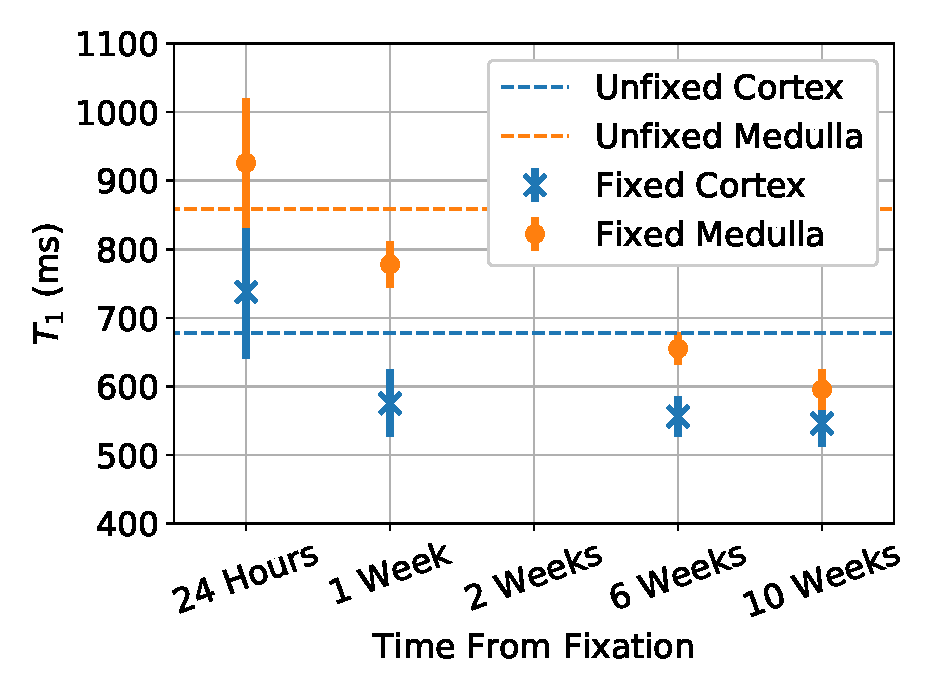
\includegraphics[width=1\textwidth]{Neph/T1_3T_crop.eps}
			\caption{}
			\label{fig:ex_fixation_t1_3t_lts}
		\end{subfigure}
		\hfill
		\begin{subfigure}[c]{0.47\textwidth}
			\centering
			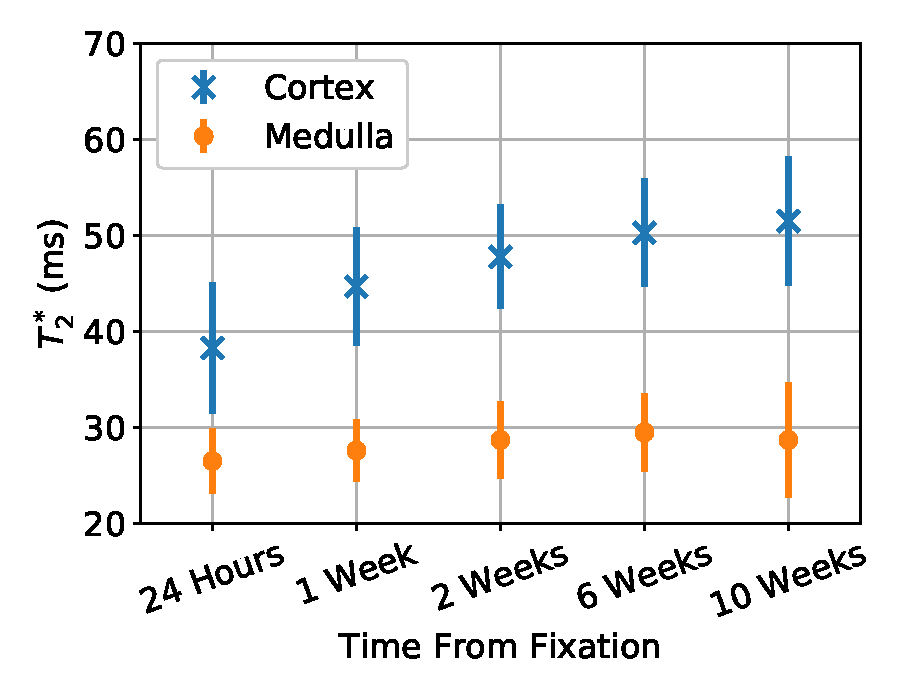
\includegraphics[width=1\textwidth]{Neph/T2star_3T_crop.eps}
			\caption{}
			\label{fig:ex_fixation_t2star_3t_lts}
		\end{subfigure}
	\end{subfigure}
	\vskip\baselineskip
	\begin{subfigure}[c]{0.9\textwidth}
		\centering
		\begin{subfigure}[c]{0.47\textwidth}
			\centering
			\includegraphics[width=1\textwidth]{Neph/T1_7T_crop.eps}
			\caption{}
			\label{fig:ex_fixation_t1_7t_lts}
		\end{subfigure}
		\hfill
		\begin{subfigure}[c]{0.47\textwidth}
			\centering
			\includegraphics[width=1\textwidth]{Neph/T2star_7T_crop.eps}
			\caption{}
			\label{fig:ex_fixation_t2star_7t_lts}
		\end{subfigure}
	\end{subfigure}
	\caption{(\subref{fig:ex_fixation_t1_3t_lts}) Variation in $T_1$ as a function of time after fixation measured at 3T (\subref{fig:ex_fixation_t2star_3t_lts}) Variation in $T_2^*$ as a function of time after fixation measured at 3T (\subref{fig:ex_fixation_t1_7t_lts}) Variation in $T_1$ as a function of time after fixation measured at 7T (\subref{fig:ex_fixation_t2star_7t_lts})  Variation in $T_2^*$ as a function of time after fixation measured at 7T.}
	\label{fig:ex_fixation_lts}
\end{figure}

\begin{figure}[H]
	\centering
	\begin{subfigure}[c]{0.47\textwidth}
		\centering
		\includegraphics[width=1\textwidth]{Neph/T1_map_STS.eps}
		\caption{}
		\label{fig:ex_fixation_t1map_3t_sts}
	\end{subfigure}
	\hfill
	\begin{subfigure}[c]{0.47\textwidth}
		\centering
		\includegraphics[width=1\textwidth]{Neph/T2star_map_STS.eps}
		\caption{}
		\label{fig:ex_fixation_t2starmap_3t_sts}
	\end{subfigure}
	\caption{(\subref{fig:ex_fixation_t1map_3t_sts}) An example of the $T_1$ map collected from the short time scale kidney (\subref{fig:ex_fixation_t2starmap_3t_sts}) An example of the $T_2^*$ map collected from the short time scale kidney.}
	\label{fig:ex_maps_sts}
\end{figure}

\begin{figure}[H]
	\centering
	\begin{subfigure}[c]{0.47\textwidth}
		\centering
		%		\missingfigure{T1 vs Times (STS)}
		\includegraphics[width=1\textwidth]{Neph/STS_T1_line.eps}
		\caption{}
		\label{fig:ex_fixation_t1_3t_sts}
	\end{subfigure}
	\hfill
	\begin{subfigure}[c]{0.47\textwidth}
		\centering
		%		\missingfigure{T2* vs Times (STS)}
		\includegraphics[width=1\textwidth]{Neph/STS_T2star_line.eps}
		\caption{}
		\label{fig:ex_fixation_t2star_3t_sts}
	\end{subfigure}
	\caption{(\subref{fig:ex_fixation_t1_3t_sts}) Variation in $T_1$ as a function of time after fixation measured at 3T (\subref{fig:ex_fixation_t2star_3t_sts}) Variation in $T_2^*$ as a function of time after fixation measured at 3T.}
	\label{fig:ex_fixation_sts}
\end{figure}

\begin{figure}[H]
	\centering
	\begin{subfigure}[c]{0.47\textwidth}
		\centering
		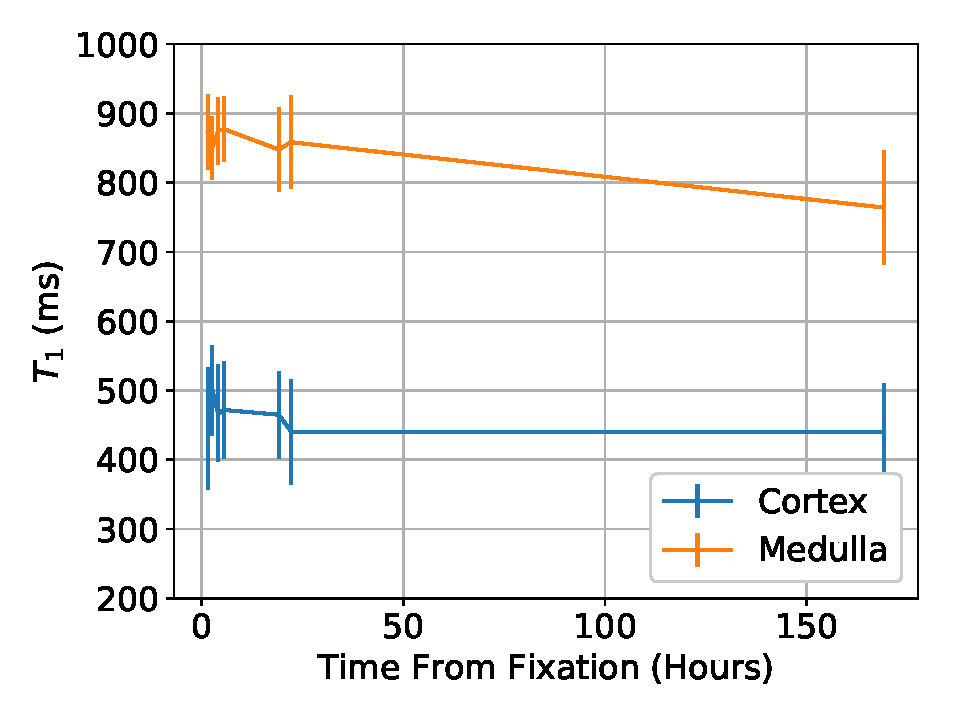
\includegraphics[width=1\textwidth]{Neph/MTS_T1_line.eps}
		\caption{}
		\label{fig:ex_fixation_t1_3t_mts}
	\end{subfigure}
	\hfill
	\begin{subfigure}[c]{0.47\textwidth}
		\centering
		\includegraphics[width=1\textwidth]{Neph/MTS_T2star_line.eps}
		\caption{}
		\label{fig:ex_fixation_t2star_3t_mts}
	\end{subfigure}
	\caption{(\subref{fig:ex_fixation_t1_3t_mts}) Variation in $T_1$ as a function of time after fixation measured at 3T (\subref{fig:ex_fixation_t2star_3t_mts}) Variation in $T_2^*$ as a function of time after fixation measured at 3T.}
	\label{fig:ex_fixation_mts}
\end{figure}
\section{Layer Based Analysis of Renal Data}
% Motivation
% Methods
% Results
\begin{figure}[H]
	\centering
	\begin{subfigure}[c]{0.47\textwidth}
		\centering
		\includegraphics[height=1\textwidth]{Other/Layers/mri_to_roi_to_surf_Artboard_5.eps}
		\caption{}
		\label{fig:ex_layers_brain}
	\end{subfigure}
	\hfill
	\begin{subfigure}[c]{0.47\textwidth}
		\centering
		\includegraphics[height=1\textwidth]{Other/Layers/kidney_levelsets-02.eps}
		\caption{}
		\label{fig:ex_layers_kidney}
	\end{subfigure}
	\caption{(\subref{fig:ex_layers_brain}) A depth mask of the brain. Lighter areas are deeper inside the brain. (\subref{fig:ex_layers_kidney}) A depth mask applied to a quantitative $T_1$ map.}
	\label{fig:ex_layers_example}
\end{figure}

\section{Correlating MRI Measures with Histopathology in Aged Kidneys}
% Method
% Results

\begin{figure}[H]
	\centering
	\begin{subfigure}[c]{0.47\textwidth}
		\centering
		\includegraphics[width=1\textwidth]{Neph/aged_kidneys/Young_T1.eps}
		\caption{}
		\label{fig:ex_aged_t1_map}
	\end{subfigure}
	\hfill
	\begin{subfigure}[c]{0.47\textwidth}
		\centering
		\includegraphics[width=1\textwidth]{Neph/aged_kidneys/Old_T1.eps}
		\caption{}
		\label{fig:ex_aged_t2star_map}
	\end{subfigure}
	\caption{(\subref{fig:ex_aged_t1_map}) $T_1$ map of a 0.5 year old pig kidney. (\subref{fig:ex_aged_t2star_map}) $T_1$ map of a 2.5 year old pg kidney.}
	\label{fig:ex_aged_map}
\end{figure}

\begin{figure}[H]
	\centering
	\begin{subfigure}[c]{0.47\textwidth}
		\centering
		\includegraphics[width=1\textwidth]{Neph/aged_kidneys/T1_bar.eps}
		\caption{}
		\label{fig:ex_aged_t1_bar}
	\end{subfigure}
	\hfill
	\begin{subfigure}[c]{0.47\textwidth}
		\centering
		\includegraphics[width=1\textwidth]{Neph/aged_kidneys/T2star_bar.eps}
		\caption{}
		\label{fig:ex_aged_t2star_bar}
	\end{subfigure}
	\caption{(\subref{fig:ex_aged_t1_bar}) The $T_1$ of the renal cortex and medulla of the two samples. (\subref{fig:ex_aged_t2star_bar}) The $T_2^*$ of the renal cortex and medulla of the two samples.}
	\label{fig:ex_aged_bar}
\end{figure}

\begin{figure}[H]
	\centering
	\begin{subfigure}[c]{0.9\textwidth}
		\centering
		\begin{subfigure}[c]{0.47\textwidth}
			\centering
			\includegraphics[width=1\textwidth]{Neph/aged_kidneys/Figure_5_V3_Young_H_and_E.png}
			\caption{}
			\label{fig:ex_young_h_and_e}
		\end{subfigure}
		\hfill
		\begin{subfigure}[c]{0.47\textwidth}
			\centering
			\includegraphics[width=1\textwidth]{Neph/aged_kidneys/Figure_5_V3_Old_H_and_E.png}
			\caption{}
			\label{fig:ex_old_h_and_e}
		\end{subfigure}
	\end{subfigure}
	\vskip\baselineskip
	\begin{subfigure}[c]{0.9\textwidth}
		\centering
		\begin{subfigure}[c]{0.47\textwidth}
			\centering
			\includegraphics[width=1\textwidth]{Neph/aged_kidneys/Figure_5_V3_Young_Trichrome.png}
			\caption{}
			\label{fig:ex_young_trichrome}			
		\end{subfigure}
		\hfill
		\begin{subfigure}[c]{0.47\textwidth}
			\centering
			\includegraphics[width=1\textwidth]{Neph/aged_kidneys/Figure_5_V3_Old_Trichrome.png}
			\caption{}
			\label{fig:ex_old_trichrome}
		\end{subfigure}
	\end{subfigure}
	\caption{(\subref{fig:ex_young_h_and_e}) A sample of renal cortex from a 0.5 year old pig stained with \ac{H and E}. (\subref{fig:ex_old_h_and_e}) A sample of renal cortex from a 2.5 year old pig stained with \ac{H and E}. (\subref{fig:ex_young_trichrome}) A sample of renal cortex from a 0.5 year old pig stained with Masson's trichrome. (\subref{fig:ex_old_trichrome}) A sample of renal cortex from a 2.5 year old pig stained with Masson's trichrome.} 
	\label{fig:ex_aged_histo}
\end{figure}

\section{Conclusion}

\section{Acknowledgements}

We are grateful for access to the University of Nottingham's Augusta high performance computing service.

\newpage
\section{References}
\defbibheading{bibliography}[\refname]{}
\printbibliography